\subsection{Integrated sampling decision}
\begin{equation}
 \boxed{f_B=\BandEdgeHz\,\mathrm{Hz}
 \ \Longrightarrow\ f_s>2f_B=12000\,\mathrm{Hz}
 \ \xrightarrow{\ f_s=F_0/M,\ M=3\ }\ f_s=\TransmissionRate\,\mathrm{Hz}.}
 \label{eq:decision-chain}
\end{equation}
The last arrow is a design choice: the measured 6 kHz edge, tested
16 kHz recovery and 12/8 kHz failure evidence justify it, with the payload
and untested-alternative costs stated above.

\begin{figure}[!htbp]
 \centering
 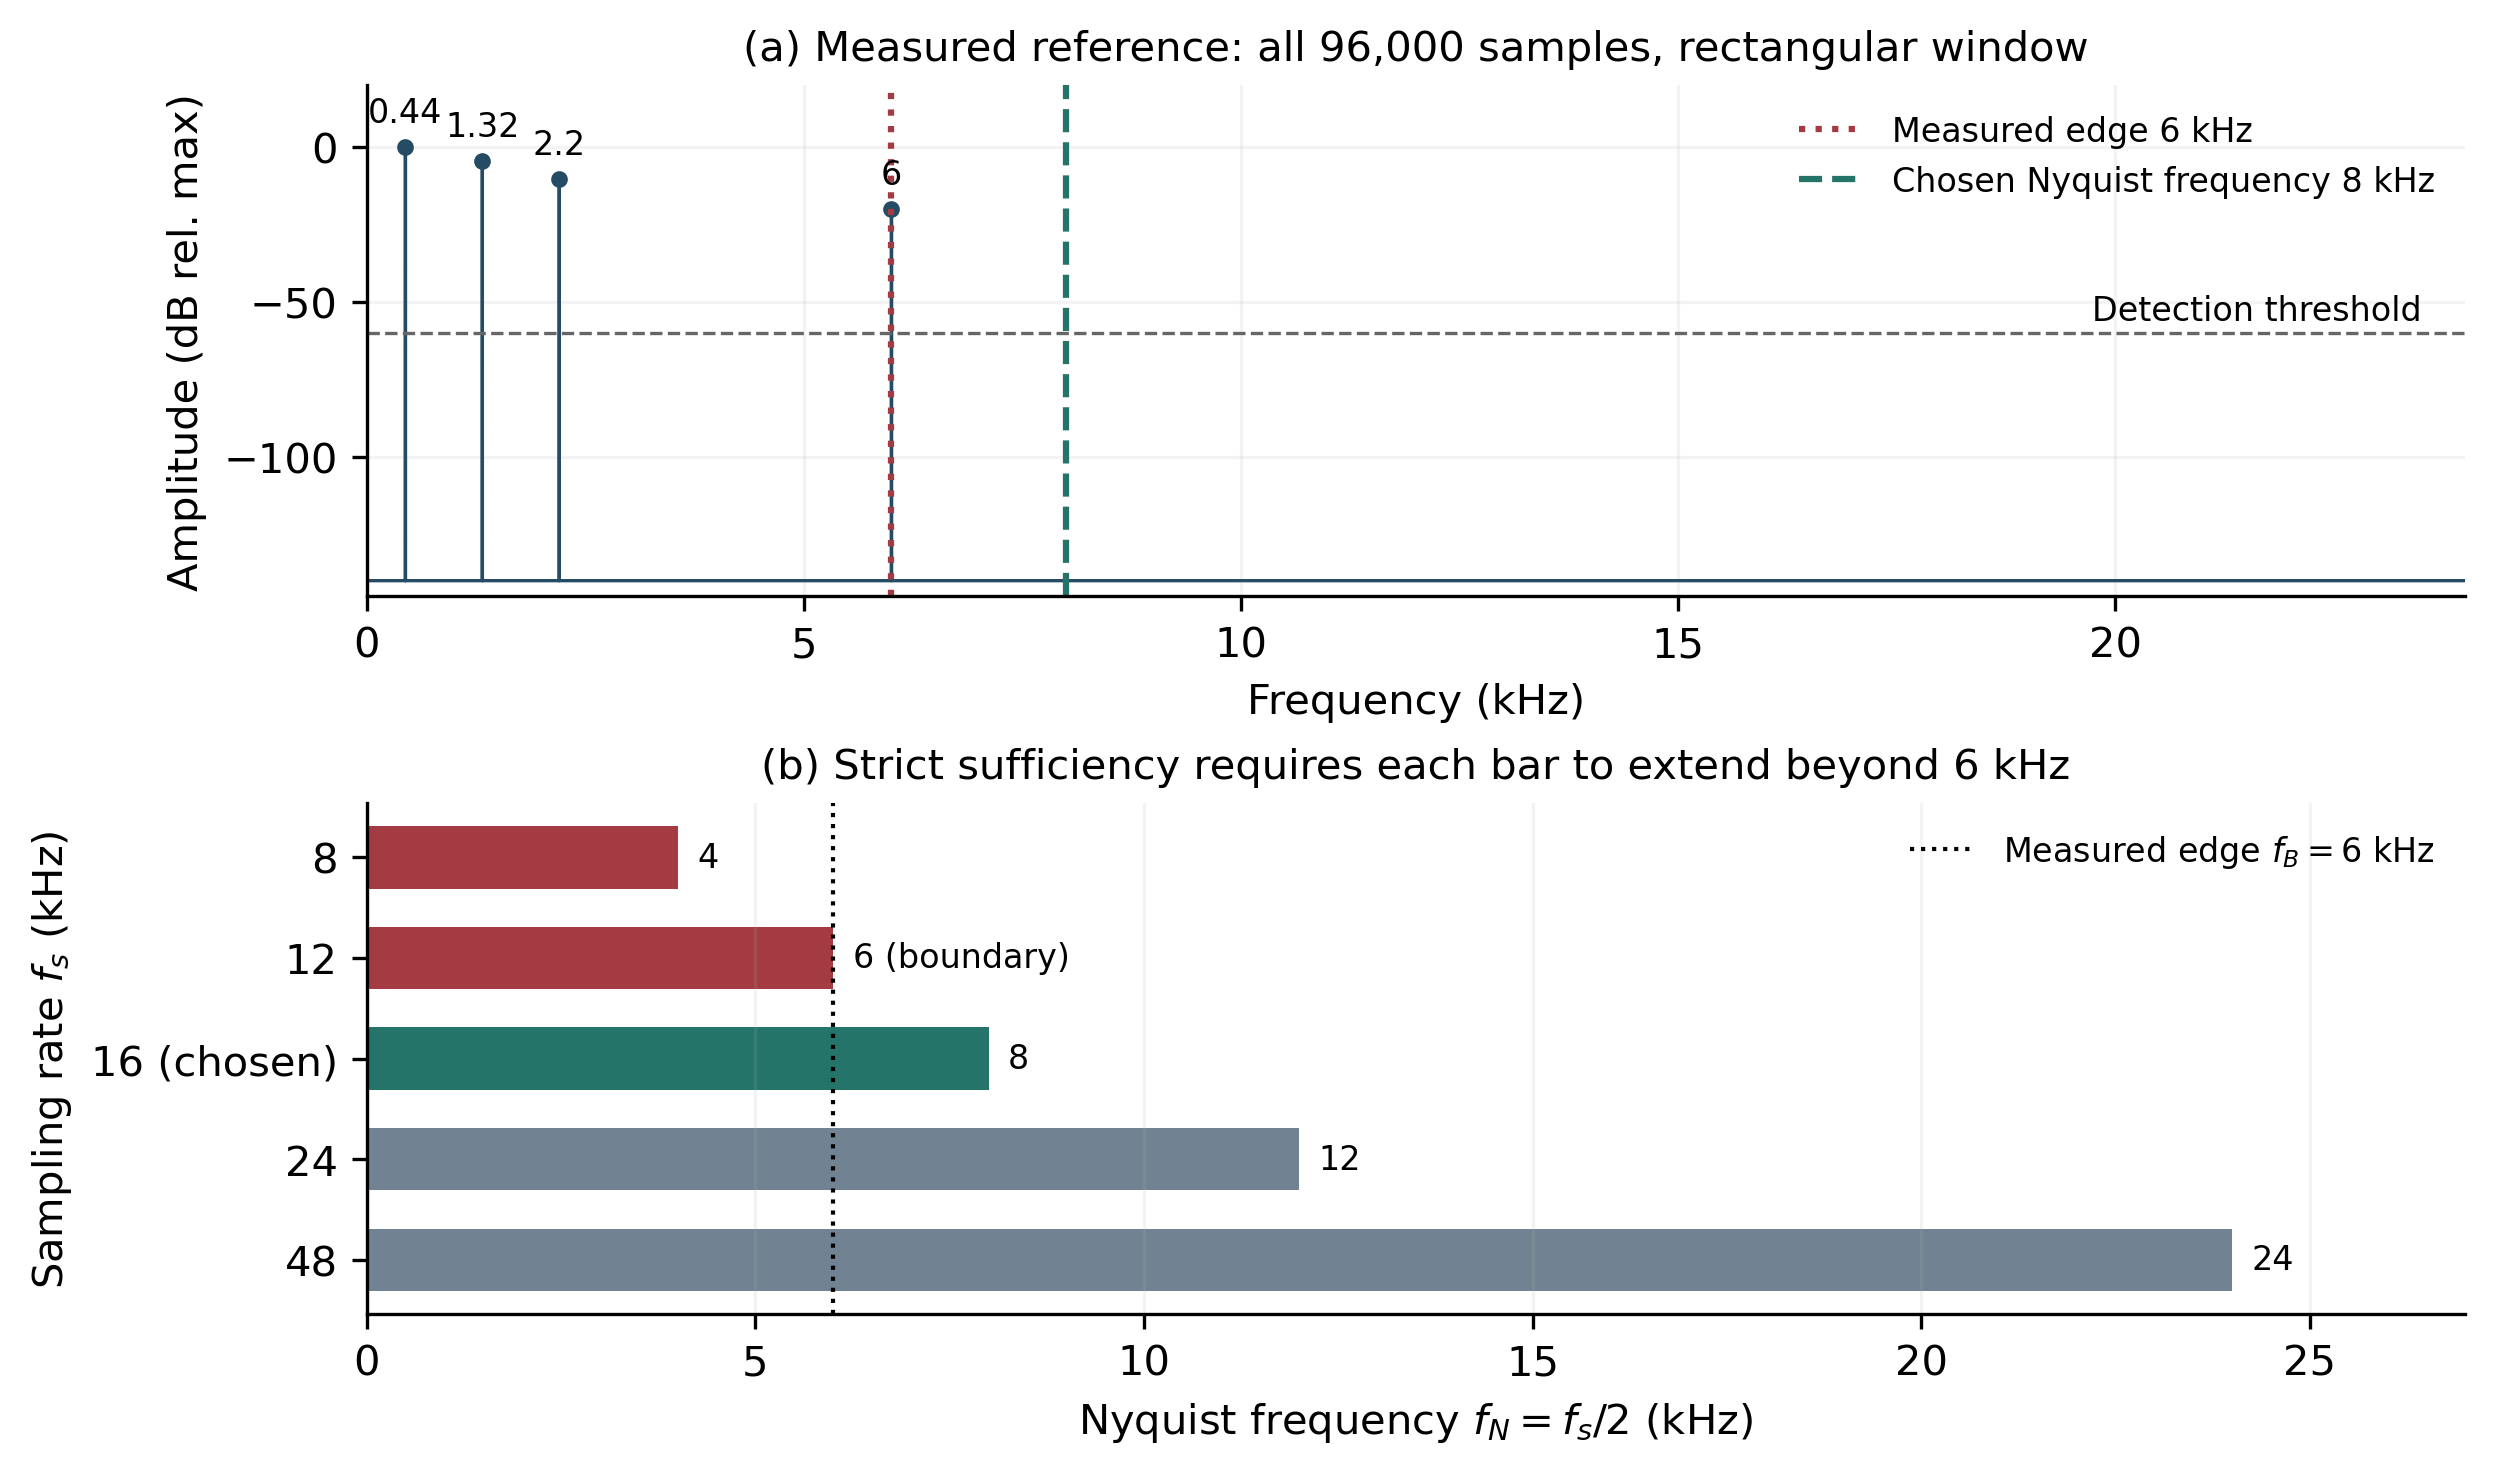
\includegraphics[width=.76\linewidth]{images/sampling_decision.png}
 \caption{Integrated R1 evidence: full-reference spectrum and candidate Nyquist limits. Peak labels use kHz; the $-60 $ dB detector and $-140 $ dB display floor have separate roles. The selected sampler leaves a 2 kHz guard.}
 \label{fig:sampling-summary}
\end{figure}

\path{stage1/r14/results/decision_summary.csv} joins
the five existing rates; six cross-stage checks and seven input hashes
verify this reporting join, which introduces no new measurements.
